\documentclass{article}
\usepackage{arxiv}

\usepackage[utf8]{inputenc}
\usepackage[english, russian]{babel}
\usepackage[T1]{fontenc}
\usepackage{url}
\usepackage{booktabs}
\usepackage{amsfonts}
\usepackage{nicefrac}
\usepackage{microtype}
\usepackage{lipsum}
\usepackage{graphicx}
\usepackage{natbib}
\usepackage{doi}
\usepackage[table]{xcolor}
\usepackage{hyperref}
\usepackage{amsmath}



\title{ALBERT for Question Answering on SQuAD 2.0}

\author{ 
	\textbf{Тохчуков Данил} \\
        Факультет вычислительной математики и кибернетики \\
        МГУ имени М. В. Ломоносова \\
	\texttt{danilkes@ya.ru} \\
}
\date{2023}

\renewcommand{\shorttitle}{}

\begin{document}
\maketitle

\begin{abstract}
    Вопросно-ответные системы используются для того, чтобы помочь людям эффективно находить релевантную информацию.
    В данной статье решается задача Question Answering на датасете SQuAD 2.0. Рассматриваются основые вопросно-ответные системы и применение их к датасету SQuAD 2.0. Среди существующих вопросно-ответных систем рассматриваются SOTA системы на основе предобученного трансформера ALBERT, и вопросно-ответная система Bidirectional Attention Flow (BIDAF). В статье предлагается собственная вопросно-ответная система на базе ALBERT и Bidirectional Attention Flow (BIDAF). Система сохраняет логику BIDAF и использует идеи из SOTA систем на базе ALBERT.
\end{abstract}

\keywords{Question Answering System \and SQuAD 2.0 \and ALBERT \and BIDAF}
\nocite{*}

\section{Введение}

Вопросно-ответные системы обычно используются для создания диалоговых клиентских приложений, 
к которым относятся приложения для социальных сетей, чат-боты и настольные приложения 
с поддержкой речи. Клиентским приложением, основанным на вопросно-ответных системах, может быть любое 
диалоговое приложение, которое общается с пользователем на естественном языке, чтобы ответить на 
вопрос.

Для того чтобы замерять качество систем, необходимы датасеты с размеченными вопросами и 
ответами. Также необходим "бенчмарк" человека -- точность ответов на вопросы, на которые он ответил.
Одним из лучших датасетов для измерения качества вопросно-ответных систем является 
SQuAD 2.0~\cite{SquadPaper} (Stanford Question Answering Dataset 2.0). 
Будем использовать его для сравнения и контроля качества систем.

\section{Постановка задачи}

\subsection{SQuAD 2.0}

\texttt{Stanford Question Answering Dataset} (SQuAD) -- это набор данных о понимании прочитанного, состоящий из вопросов, задаваемых краудворкерами в наборе статей Википедии, где ответом на каждый вопрос является фрагмент текста из соответствующего контекста, или вопрос может быть без ответа.

Целью систем, использующих набор данных SQuAD 2.0, должно быть не только отвечать на вопросы, когда это возможно, но и определять, когда абзац не подкрепляет ответ, и воздерживаться от ответа.

Датасет состоит из 130,319 объектов обучающей выборки и 11,873 объектов тестовой выборки. В обучающей выборке 33\% объектов не имеют ответа на вопрос, в валидационной же 50\% объектов без ответа.

Каждый объект представляет из себя контекст, вопрос и ответ: Рис.~\ref{fig:squad}.

\begin{figure}[!ht]
    \centering
    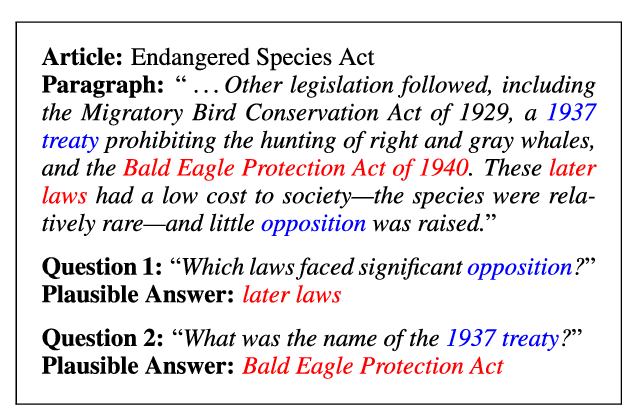
\includegraphics[width=150mm]{../figures/squad_example.png}
    \caption{Пример из SQuAD 2.0}
    \label{fig:squad}
\end{figure}

\subsection{Задача классификации}

Задача состоит в том, чтобы найти правильный ответ на заданный вопрос по тексту, 
причём ответ на вопрос непрерывен и целиком находится в тексте -- это значит что он не разделяется
другими токенами из текста. \textit{Токен} -- небольшая часть текста, 
находящаяся в определенном месте этого текста и имеющую определенное значение (простой пример -- слово).
Учитывая факт непрерывности, будем предсказывать индекс первого и последнего токена ответа в тексте,
то есть будем находить подстроку, являющуюся ответом на поставленный вопрос.

Если в тексте не будет искомого ответа, модель должна вывести что ответа нет.

Итого, имеется задача классификации для начального и конечного токенов ответа, с одним только ограничением,
что токен конца ответа не может стоять перед токеном начала.

\subsection{Метрики}

Для измерения качества моделей применяются две метрики: Exact Match (EM) score и F1
score.

\texttt{Exact Match} это двоичная мера (истина/ложь) того, точно ли выходные данные системы соответствуют
основному истинному ответу (exact match accuracy). Это довольно строгий показатель.

\texttt{F1} менее строгая метрика. Это среднее гармоническое precision и recall модели. \\
$$F1 = 2*\frac{\text{precision}*\text{recall}}{\text{precision} + \text{recall}}$$

Система должна набирать наибольшее значение качества по метрикам EM и F1.

\section{Существующие системы}

Всего систем для задачи Question Answering довольно много, но будут рассмотрены лишь некоторые из них
Для датасета SQuAD 2.0 одни из лучших систем были на базе трансформерной модели 
BERT от Google AI~\cite{BERTPaper}. На основе BERT было сделано много моделей в 2019 году, и считались state of the art решением~\cite{BERTsquad}. Однако в 2020 году вышел ALBERT~\cite{ALBERT} и теперь одни из самых лучших систем построены именно на ALBERT.

\subsection{ALBERT}
A Lite BERT(ALBERT) -- такая же языковая модель с механизмом Self-Attention~\cite{Attention} как и BERT, но отличается от BERT тем, что он легче, быстрее обучается и использует несколько приёмов, в их числе факторизация эмбеддингов, что в теории должно пропускать через слои больше информации о контексте токенов.

\begin{figure}[!ht]
    \centering
    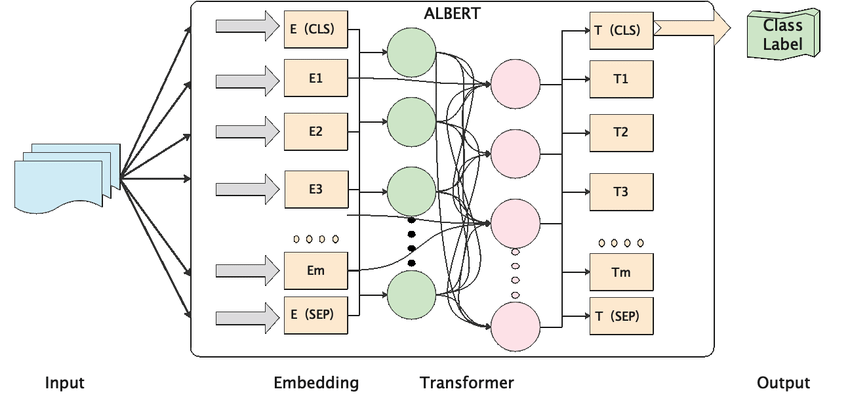
\includegraphics[width=150mm]{../figures/ALBERT.png}
    \caption{Архитектура ALBERT}
    \label{fig:albert}
\end{figure}

Существуют работы на базе ALBERT для SQuAD 2.0, например ALBERT (ensemble)~\cite{ALBERTsquad}. В ней контекст объединяется с запросом через токен-разделитель и используется предобученный ALBERT для получения эмбеддингов. Затем используется ансамбль нескольких моделей, которые используют стек из RNN, Attention, Self Attention и BIDAF-out (речь о котором пойдёт ниже).

\begin{figure}[!ht]
    \centering
    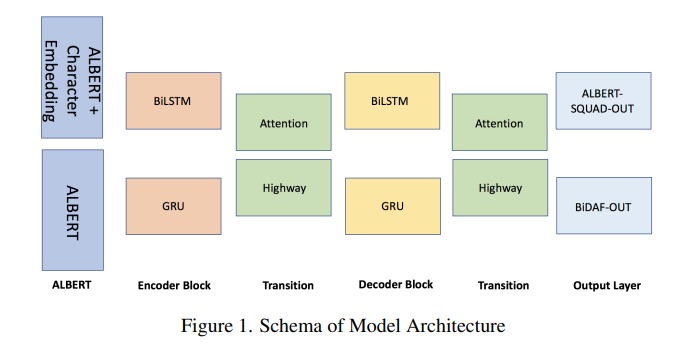
\includegraphics[width=150mm]{../figures/ALBERTsquad.png}
    \caption{ALBERT (ensemble) system for SQUAD 2.0}
    \label{fig:albertsquad}
\end{figure}

Работа до сих пор остаётся одной из лучших в рейтинге SQuAD 2.0, однако модель, которую они предлагают является довольно крупной и труднообучаемой в силу большого количесва Attention и bi-LSTM слоёв.
ALBERT, как и BERT, может строить контекстно зависимые признаки, при этом он обучен на большом количестве данных, поэтому его очень хорошо использовать для построения эмбеддингов.

\subsection{BIDAF}

Рассмотрим модель Bi-Directional Attention Flow (BIDAF)~\cite{BIDAF}. Это полноценная вопросно-ответная систем, которая показала отличное качество на SQuAD 1.0~\cite{SQuADfirst}
Устройство её работы представлена на схеме:

\begin{figure}[!ht]
    \centering
    \includegraphics[width=150mm]{../figures/BIDAF.png}
    \caption{BIDAF}
    \label{fig:bidaf}
\end{figure}

Суть работы модели заключается в том, что в ней авторы получают эмбеддинги с помощью GloVe~\cite{glove}, затем прогоняют их через bi-LSTM, а дальше отправляют эмбеддинги вопроса и контекста в Bidirectional Attention слой, где вычисляется Attention от "запроса" вопроса к ключам контекста, и наоборот. Затем выход Attention слоя отправляется на вход очередной bi-LSTM. Затем, с помощью линейных слоёв, bi-LSTM и softmax получают вероятности начального и конечного токена в контексте (start, end).
BIDAF также хорошо используется в ансамбле, например как в этой работе с BERT~\cite{BERTbidaf}.

\section{Предложенная система}

BIDAF обладает недостатками, которые можно улучшить. Система использует контекстно-независимые эмбеддинги Glove и подаёт их на вход bi-LSTM, чтобы найти контекстную связь между токенами. У этого подхода есть проблема затухания сигнала, ведь bi-LSTM -- рекурентная суть, а значит сигнал с дальних участков текста может не дойти до некоторых токенов. Чтобы исправить это, используем вместо GloVe + bi-LSTM предобученный ALBERT -- он уловит контекст и построит контекстно-зависимые эмбеддинги для исходного вопроса и для контекста (отдельно).

Построенные эмбеддинги вопроса и контекста отправляются в bi-GRU, чтобы закодировать токены, а затев в Query2Context (Attention) слой, который будет показывать насколько контекст соответствуют вопросу. Далее выход bi-GRU отправляется в декодер, а затем в кастомный BIDAF-out из статьи~\cite{ALBERTsquad}, отличие в том, что в нём используется GRU.

\begin{figure}[!ht]
    \centering
    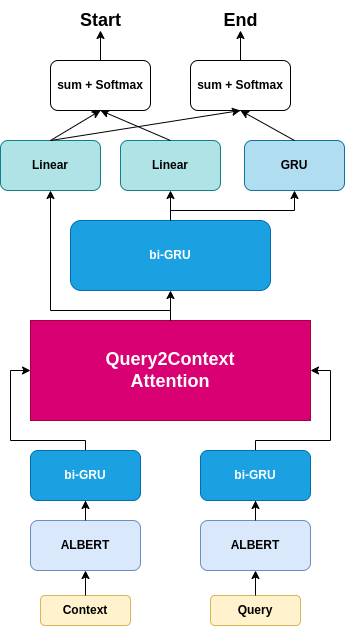
\includegraphics[width=50mm]{../figures/model_diagram.drawio.png}
    \caption{Предложенная QA система}
    \label{fig:customqa}
\end{figure}

Такой подход позволяет облегчить модель из статьи~\cite{ALBERTsquad}, сохраняя при этом логику BIDAF. Таким образом, мы построили вопросно-ответную систему, у которой исправлены недостатки BIDAF и при этом облегчен размер модели из~\cite{ALBERTsquad}.

\section{Реализация}

Для начала необходимо создать embeddings с помощью ALBERT. Для этого необходимо обязательно убрать из SQuAD 2.0 те данные, кодировка которых будет по длине больше 512. Дело в том, что у ALBERT (как и у BERT) стоит ограничение на длину последовательности (в токенах) в целях экономии ресурсов и времени работы модели. Embeddings получаются прямым проходом закодированных текстов через ALBERT (у ALBERT свой кодировщик входной последовательности).

Чтобы модель могла определять что в контексте ответа нет, будем добавлять в начало контекста спец. токен. Для объектов, у которых нет ответа на вопрос из контекста индекс начала и конца токена ответа будем ставить на спец. токен.

Дальше модель строится на базе pytorch по блокам как изображено на блок-схемы.

\section{Результаты и сравнение систем}

\begin{table}[h]
    \centering
    \begin{tabular} {|c|c|c|c|}
        \hline
        \multicolumn{4}{|c|}{SQuAD 2.0} \\
        \hline
        Модель & custom & ALBERT(ensemble) & BIDAF\\
        \hline
        EM & - & 89.731 & 63.372\\
        \hline
        F1 & - & 92.215 & 66.251 \\ 
        \hline
    \end{tabular}
\end{table}

После прохода эмбеддингов по модели, мы получаем распределения для токенов -- для start и end. Ниже приведён пример: распределения start/end после работы модели на вопросе: "How many parameters does BERT-Large have?": Рис.\ref{fig:starttoken}, Рис.\ref{fig:endtoken}.

\begin{figure}[!ht]
    \centering
    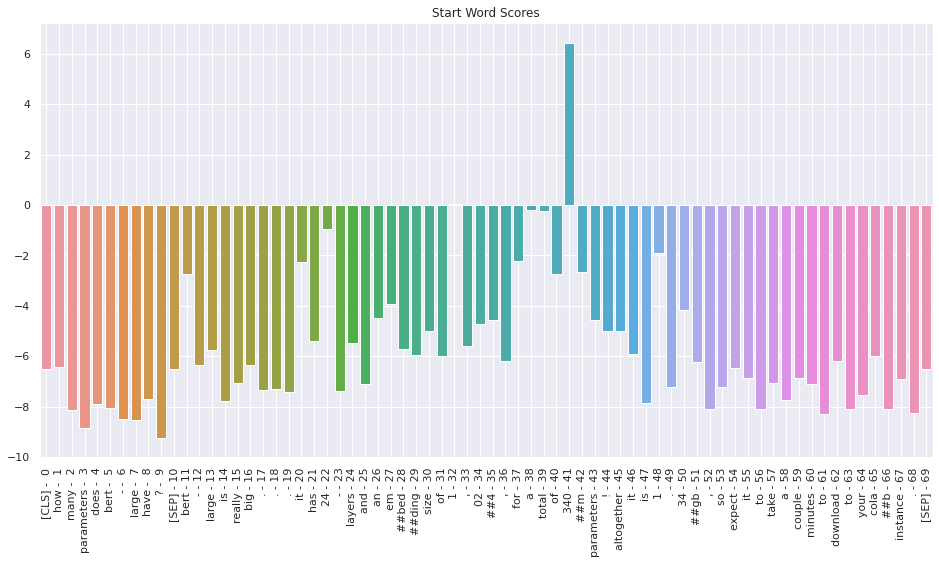
\includegraphics[width=120mm]{../figures/start_token.png}
    \caption{Start token scores}
    \label{fig:starttoken}
\end{figure}

\begin{figure}[!ht]
    \centering
    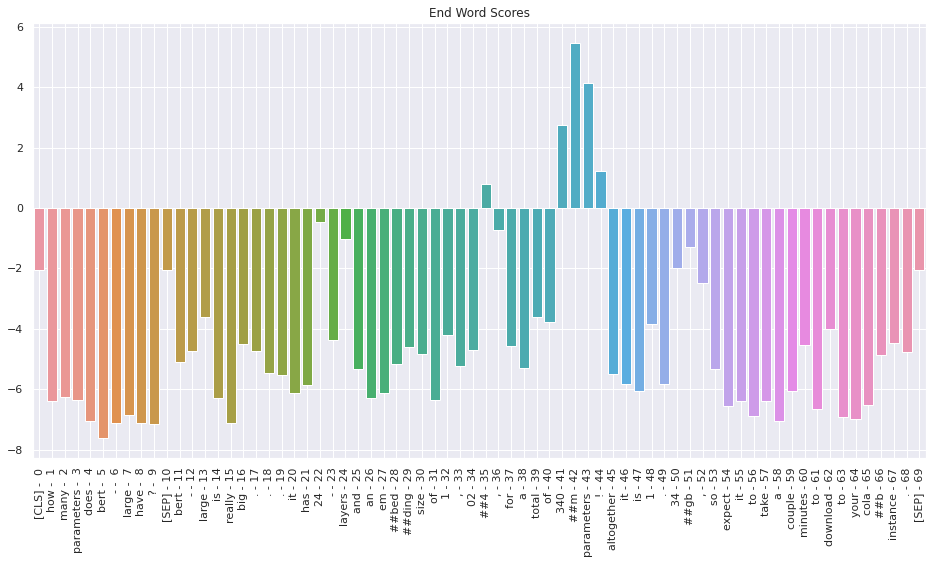
\includegraphics[width=120mm]{../figures/end_token.png}
    \caption{End token scores. Answer is "340m"}
    \label{fig:endtoken}
\end{figure}

\section{Заключение}

Question Answering Systems (QAS) сегодня достигают результатов, сравнимых с человеческими, и всё благодаря таким предобученным моделям как BERT, ALBERT, GPT. На их основе создаются решения многих NLP задач, в том числе и решения для задачи нахождения ответов на вопросы по тексту.

Итого, в работе была решена задача Question Answering на датасете SQuAD 2.0. Также в работе были представлены основные существующие системы на базе трансформеров для решения Question Answering задачи. Также была предложена архитектура "облегченной" вопросно-ответной системы на базе трансформера ALBERT.

\subsection{Дальнейшие улучшения}
Заметим, что изначально в BIDAF использовался GloVe и CharCNN для эмбеддингов, таким образом мы могли дробить слова на составные части и кодировать их. ALBERT тоже дробит слова, но гораздо меньше. Чтобы увеличить информацию о составных частях слов, хорошей практикой будет добавить эмбеддинги букв к исходным эмбеддингам и обучаться на них.

\bibliographystyle{abbrv}
\bibliography{references}

\end{document}
